\documentclass[10pt]{jarticle}
\usepackage{float}
\usepackage{adrobo_abst}
\usepackage[dvipdfmx]{graphicx}
\usepackage{amssymb,amsmath}
\usepackage{bm}
\usepackage[superscript]{cite}
\usepackage{enumerate}
\usepackage{url}
%\usepackage[absolute]{textpos}

\renewcommand\citeform[1]{(#1)}

\begin{document}
    
    \makeatletter
    \doctype{2020年度卒業論文概要}
  \title{カメラ画像と目標方向を用いたEnd-to-End学習によるシナリオに基づくNavigation手法の提案}{(カメラ画像と目標方向による予備実験)}
    \etitle{Making Research Paper}{($\bigcirc\bigcirc\bigcirc$)}
    
    \author{18C1096\hspace{.5zw}春山健太}
    \eauthor{Kenta HARUYMA}
    
    \makeatother
    
    \abstract{When preparing the manuscript, read and observe carefully this sample as well as the instruction manual for the manuscript of the Transaction of Japan Society of Mechanical Engineers. This sample was prepared using MS-word. Character size of the English title is 14 pts of Times New Roman as well as sub-title. The name is 12 pts. The address of the first author and the abstract is 10 pts of Times New Roman. Character spacing of the abstract is narrowed by 0.2 pts preferably.}
    
    \keywords{End-to-End, Navigation, Target Direction}
    
    \maketitle
    
    \supervisor{指導教員:林原靖男 教授}
    
    \section{緒\hspace{2zw}言}%===========================
    近年,様々なセンサを用いた移動ロボットの自律移動に関する研究が盛んに行われており,
    その中でカメラ画像を用いてロボットへ自律移動を行わせる研究も行われている.
    Bojaskiら\cite{nvidia}は人間のハンドル操作によるステアリングの
    角度の模倣学習を行い,画像を用いて走行を行う方法を提案している.

    また岡田ら\cite{okada}はLiDARとオドメトリを入力とするルールべースの制御器を用いて自律移動を行い,
    その制御器の出力する角速度とロボットに取り付けたカメラから取得したカメラ画像を用いて
    学習器の訓練を行い,学習後はカメラ画像のみを用いて自律移動を行う.
    ルールベースの制御器を用いることでデータセットを自動的に収集し,
    その経路追従行動を模倣する手法を提案している.
    上記の研究により,カメラ画像を用いたEnd-to-End学習によって
    ロボットが一定の経路を周回することが可能であると示されている.
    
    次に上記の研究を拡張し,経路内に\reffig{bunki}のような分岐路において,
    赤で示す「直進」と緑で示す「左折」の経路を選択する手法を考える.
    カメラ画像のみでは必要な情報が不足していると考えられる.
    そこで,データセットへカメラ画像以外に「右折」「左折」などの目標とする方向の情報
     ( 本研究では”目標方向”とする )を追加することで分岐路において特定のルートを選択することが可能であると考えられる.

    本稿ではカメラ画像と目標方向を入力とするEnd-to-End学習による走行において,目標方向によって
    分岐路で任意のルートへ走行経路を変更が可能であるかの検証を行う.
    \begin{center}
        \begin{figure}[h]
            \centering
            \includegraphics[width=0.3\textwidth]{./fig/bunki.pdf}
            \caption{Cross road}
            \label{fig:bunki}
        \end{figure}
    \end{center}
    \section{提案手法}%===========================
    提案手法を学習器の訓練を行う「学習フェーズ」,訓練した学習器の出力を用いて走行する「テストフェーズ」
    の2つに分けて述べる.
    % \subsection{学習フェーズ}
    
    学習フェーズで用いるシステムを\reffig{system_learning}に示す.
    地図ベースの制御器はROS Navigation\_stack\cite{navigation}へ目標方向の生成機能を追加したルールベース制御器である.
    目標方向は「continue,go straihgt,go left,go right」の4つとし,これらを要素数4のOne-hotベクトルで表現する.
    学習器の訓練は次の流れを 1stepとして自動的にデータセットを収集し,設定したstep数の学習行う.
    1)LiDAR とオドメトリから得たデータを入力とする地図ベースの制御器の出力を用いて自律走行を行う.
    2)地図ベースの制御器の出力からヨー方向の角速度と目標方向,機体に取り付けた3つのカメラから
    RGB画像を取得し,訓練データへ加える.
    3)訓練データ(入力:カメラ画像,目標方向 目標出力:角速度)を用いてEnd-to-End学習を行い,学習器の出力を記録.

    \begin{center}
        \begin{figure}[h]
            \centering
            \includegraphics[width=0.40\textwidth]{./fig/system_learning.pdf}
            \caption{Learning phase}
            \label{fig:system_learning}
        \end{figure}
    \end{center}
    
    % \subsection{テストフェーズ}
    
    設定したstep数に達した場合に, テストフェーズへ移行し,
    \reffig{system_test}に示すように中央のカメラ画像と目標方向を入力とした
    学習器の出力(角速度)による走行を行う.
    テスト時の目標方向は Joy stickコントローラのボタンを用いて入力する.
    テストフェーズにおける手順を下記に示す.
    1)機体に取り付けた中央のカメラから RGB 画像 ,Joy stick コントローラより目標方向のデータを取得.
    2)取得したデータ (カメラ画像,目標方向) を学習器へ入力.
    3)学習器の出力(角速度)を用いて自律走行を行う.
    % \begin{enumerate}
    % \setlength{\parskip}{0cm} % 段落間
    % \setlength{\itemsep}{0cm} % 項目間
    % \item 機体に取り付けた中央のカメラから RGB 画像 ,Joy stick コントローラより目標方向の
    % データを取得
    % \item 取得したデータ ( カメラ画像,目標方向 ) を学習器へ入力
    % \item 学習器の出力(角速度)をモータへ与える
    % \end{enumerate}
    \begin{center}
        \begin{figure}[h]
            \centering
            \includegraphics[width=0.38\textwidth]{./fig/system_test.pdf}
            \caption{Test phase}
            \label{fig:system_test}
        \end{figure}
    \end{center}
    
    \section{実\hspace{2zw}験}%===========================
    実験では\reffig{system_learning},\reffig{system_test}で示すturtlebot3 waffleへカメラを3つ追加したモデルを用いる.
    環境とルートを\reffig{exp}に示す.環境はgazebo上で作成した道幅が2.5mの十字路を用い,
    ルートは2,3,4の地点に到達後,緑の初期位置へロボットの位置,自己位置推定をリセット
    を行いながら,緑-青-1,緑-青-2,緑-青-3の順で走行を行う.
    目標方向は学習フェーズ,テストフェーズともに緑-青(continue)青-赤1(go straihgt)青-赤2(go left)青-赤3(go right)を入力している.
    step数は4000stepとした.
    実験条件はテストフェーズにおいて「壁に衝突せず,目標方向に対応したコースを選択」を成功,
     「目標方向とは異なったコースを選択する,または壁に衝突」を失敗とする.
    実験結果を\reftab{suc}に示す.
    % \begin{enumerate}
    %     \setlength{\parskip}{0cm} % 段落間
    %     \setlength{\itemsep}{0cm} % 項目間
    %     \item 学習フェーズによって,学習器の訓練 ( 経路の学習 ) 行う
    %     ( 制御:地図べースの制御器の出力 )
    %     \item 設定した step 数を学習後,訓練フェーズへ移行
    %     ( 制御:学習器の出力 )
    %     \item コース内に設定した地点において目標方向のコマンドを入力,挙動を確認
       
    % \end{enumerate}
    \begin{center}
        \begin{figure}[h]
            \centering
            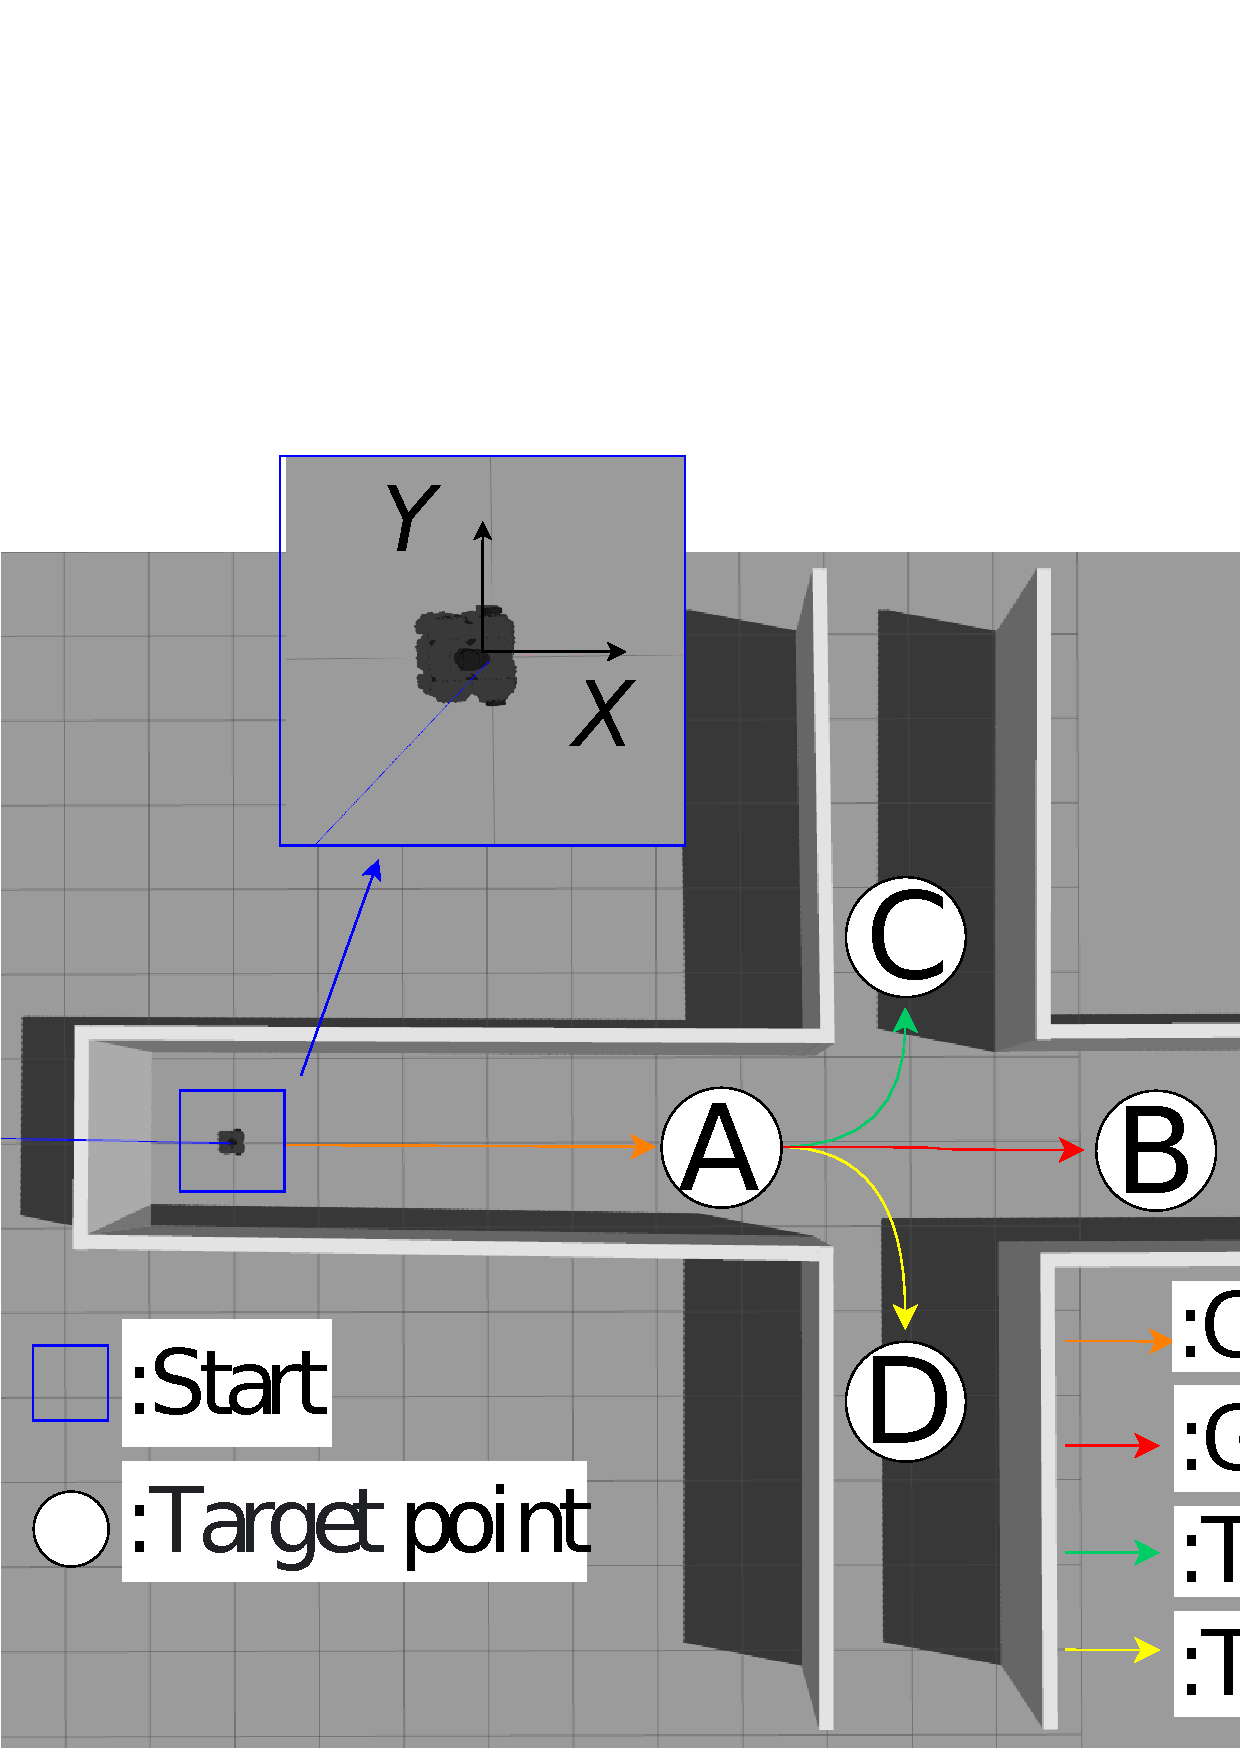
\includegraphics[width=0.34\textwidth]{./fig/zyuziroute.pdf}
            \caption{Course and route of experiment}
            \vskip 0.1zh
            \label{fig:exp}
        \end{figure}
    \end{center}
    \vspace{-1zh}
    \begin{table}[h]
        \caption{Number of successes experiment 1 point}
        \label{tab:suc}
        \begin{center}
            \vskip -1zh
            \begin{tabular}{|c|c|}
                \hline
                Target direction and Point & Number of successes\\ \hline
                continue (1) & $5/5$ \\ \hline
                go straihgt (2) & $5/5$ \\ \hline
                go left (3) & $4/5$ \\ \hline
                go right (4) & $5/5$ \\ \hline
            \end{tabular}
        \end{center}
    \end{table}
            
    \section{結\hspace{2zw}言}%===========================
    本稿ではカメラ画像と目標方向を用いたEnd-to-End学習による,
    特定のルート選択を選択可能なNavigation手法を提案し,
    実験結果から分岐路において目標方向を用いて特定のルートが選択する行動が見られた.
    
    \vspace{5truemm}
    {\footnotesize
        \begin{thebibliography}{99}
            
            % \bibitem{工大2005}
            % 工大太郎: ``ロボットのしくみ'', 
            % 日本機械学会論文誌A, 
            % Vol.~108, No.~1034 (2005), pp.~1--2.
            
            \bibitem{nvidia}
            Mariusz Bojarski et al:``End to End Learning for Self-Driving Cars'',
            arXiv: 1604.07316,(2016)
            \bibitem{okada}
            岡田眞也, 清岡優祐, 上田隆一, 林原靖男:``視覚と行動の end-to-end 
            学習により経路追従行動をオンラインで模倣する手法の提案''
            SICE-SI2020予稿集,1147--1152,制御学会SI部門講演会(2020)
            \bibitem{navigation}
            ros-planning, navigation: 
            \url{https://github.com/ros-planning/navigation}, 
            (参照日 2020年12月30日). 
            % \bibitem{Shibutani2004}
            % Y. Shibutani: ``Heinrich's Law Resulted Pattern Dynamics --Part2--'',
            % Proceedings of the 79th Kansai Branch Regular Meeting of the Japan Society of Mechanical Engineers,  
            % No.~04--05 (2004), pp.~205--206.
            
            % \bibitem{Handbook1979}
            % The Japan Society of Mechanical Engineers ed.: ``JSME Date Handbook: Heat Transfer'', 
            % (1979), p.~123, The Japan Society of Mechanical Engineers.
            
            % \bibitem{Kikuchi2017}
            % K. Kikuchi, M. Miura, K. Shibata, J. Yamamura: ``Soft Landing Condition for Stair-climbing Robot with Hopping Mechanism'', 
            % Journal of JSDE, Vol.~53, No.~8 (2018), pp.~605--614, \url{https://doi.org/10.14953/jjsde.2017.2774}.
        \end{thebibliography}
    }
    \normalsize
    
\end{document}
